\documentclass[spanish]{article}
\usepackage{graphicx}
\usepackage{ragged2e}
\usepackage{geometry}
\usepackage{float}
\usepackage{hyperref}
\usepackage[table,xcdraw]{xcolor}
\usepackage[ruled,vlined]{algorithm2e}
\title {Práctica 1: Determinación experimental de la complejidad de un algoritmo}
\graphicspath{{../img/}}
\addtolength{\textheight}{1.5in} 
\begin{document}
	\centerline{
\includegraphics[width=450px,height=100px]{header}}
	\centerline{Analisis de algoritmos, Sem: 2021-1, 3CV1,Práctica  3, 11/11/2020}
	\centering{\huge{Practica 3.  Complejidades temporales polinomiales y no polinomiales.}}
	\centerline{\newline{\textbf{Payán Téllez René}}}
	\newline{\textit{rpayant1500@alumno.ipn.mx}}
	\bigskip
	\justify
	\textbf{Resumen:}	
	En esta practica se compararan algoritmos cuya complejidad es polinomial (es decir esta acotada por un polinomio definido por "n") y algoritmos no polinomiales (es decir que no estan acotados por un polinomio).\\
	\textbf{Palabras clave:}
	Polinomial,No polinomial,Complejidad,C/C++
	\section{Introduccion}
	
	\section{Conceptos Basicos}
	\subsection{Algoritmo}
	La palabra algoritmo proviene del sobrenombre de un matemático árabe del siglo IX, Al-Khwarizmi, que fue reconocido por enunciar paso a paso las reglas para las operaciones matemáticas básicas con decimales (suma, resta, multiplicación y división).	
	Vemos definición de algoritmo como un grupo de órdenes consecutivas que presentan una solución a un problema o tarea. Algunos ejemplos de algoritmos los podemos encontrar en las matemáticas (como el algoritmo para resolver una multiplicación) y en los manuales de usuario de un aparato (como una lavadora o una impresora).	
	Sin embargo, hoy en día se relaciona la palabra algoritmo con el mundo de la informática, más concretamente en la programación; los conocidos como algoritmos informáticos.[1]
	\subsection{Complejidad algoritmica}
	Así que, por su naturaleza, un problema tiene la capacidad de ser solucionado por uno o varios métodos, pero si bien es importante llegar a la respuesta, más importante es evaluar su viabilidad. Siempre que se analiza y evalúa adecuadamente la efectividad de una solución, disminuye drásticamente el costo que representa su producción y mantenimiento, pues los recursos que se invierten posteriormente en codificación, pruebas y revisión es mucho menor siempre (como el tiempo, dinero y talento humano).	
	Entrando en materia, la complejidad algorítmica es una métrica teórica que nos ayuda a describir el comportamiento de un algoritmo en términos de tiempo de ejecución (tiempo que tarda un algoritmo en resolver un problema) y memoria requerida (cantidad de memoria necesaria para procesar las instrucciones que solucionan dicho problema). Esto nos ayuda a comparar entre la efectividad de un algoritmo y otro, y decidir cuál es el que nos conviene implementar.[2]
	\subsection{Algoritmo Polinomial}
	En computación, cuando el tiempo de ejecución de un algoritmo (mediante el cual se obtiene una solución al problema) es menor que un cierto valor calculado a partir del número de variables implicadas (generalmente variables de entrada) usando una fórmula polinómica, se dice que dicho problema se puede resolver en un tiempo polinómico.[3]	
	\subsection{Algoritmo No Polinomial}
	En teoría de la complejidad computacional, NP es el acrónimo en inglés de nondeterministic polynomial time ("tiempo polinomial no determinista"). Es el conjunto de problemas que pueden ser resueltos en tiempo polinómico por una máquina de Turing no determinista.[4]
	La importancia de esta clase de problemas de decisión es que contiene muchos problemas de búsqueda y de optimización para los que se desea saber si existe una cierta solución o si existe una mejor solución que las conocidas. En esta clase están el problema del viajante (también llamado "problema del viajante de comercio" o "problema del agente viajero") donde se quiere saber si existe una ruta óptima que pasa por todos los nodos en un cierto grafo y el problema de satisfacibilidad booleana en donde se desea saber si una cierta fórmula de lógica proposicional puede ser cierta para algún conjunto de valores booleanos para las variables.[4]
	\subsection{Sucesión de Fibonacci}
	Esta sucesión fue descrita por Fibonacci como la solución a un problema de cría de conejos: “Cierto hombre tiene una pareja de conejos juntos en un lugar cerrado y desea saber cuántos son creados a partir de este par en un año cuando, de acuerdo a su naturaleza, cada pareja necesita un mes para envejecer y cada mes posterior procrea otra pareja”[5]
	\subsection*{Solucion iterativa para encontrar el termino $N$ en la secuencia de fibonacci}
	\begin{algorithm}[H]
		\KwData{Entrada: N}
		\KwResult{Retorna el N-esimo termino de la serie de fibonacci}
		a=0\;
  	    b=0\;
  	    c=0\;
		\For{$i\gets1$ \KwTo $N$}{
			c = a\;
			a = b\;
			b += c\;
		}
		return a\;
		\caption{Solucion iterativa}
	\end{algorithm}
	\subsection*{Solucion recursiva para encontrar el termino $N$ en la secuencia de fibonacci}
	\begin{algorithm}[H]
		\KwData{Entrada: N}
		\KwResult{Retorna el N-esimo termino de la serie de fibonacci}
		\If{$N$ = 0}{
			return 0\;		
		}
		\ElseIf{$N$ = 1}{
			return 1\;
		}
		\Else{
			return 	solucionRecursiva($N$-1)+solucionRecursiva($N$-2);
		}
		\caption{Solucion recursiva}
	\end{algorithm}
	\subsection{Número perfecto}
	Si hablamos de números, un número perfecto es aquél que es igual a la suma de sus divisores, exceptuando él mismo (estos divisores que no incluyen al mismo número son los que se conocen como factores o divisores propios).[6]
	\subsection{Algoritmo para determinar si un número N es perfecto}
	\begin{algorithm}[H]
		\KwData{Entrada: N}
		\KwResult{Retorna 1 si el número es perfecto, en otro caso retorna 0}
		raiz $\gets\sqrt{N}$\;
		suma $\gets$ 1\;	
		\For{$i\gets2$ \KwTo raiz}{
			\If{n mod i = 0}{
				suma $\gets$ suma + i\;
				\If{$n/i > raiz$}{
					suma $\gets$ suma + n/i\;
				}
			}	
		}	
		\If{suma == $N$}{
			return 1\;		
		}
		\Else{
			return 0\;
		}
		\caption{Perfecto(N)}
	\end{algorithm}	
	\subsection{Algoritmo para mostrar los primeros N números perfectos}
	\begin{algorithm}[H]
		\KwData{Entrada: N}
		\KwResult{Imprime los primeros N números perfectos}
		i $\gets$6\;
		\While{$N>$0}{
			\If{Perfecto(i) = 1}{
				Imprimir(i)\;
				$N$$\gets$$N$-1\;
			}	
		}	
		\caption{MuestraPerfectos(N)}
	\end{algorithm}
	La complejidad de la funcion puede reducirse por la propiedad de los números perfectos de que estos son iguales a: $(\frac{2^p}{p})(2^p-1)$, por lo tanto si se logra reducir la complejidad para obtener números primos, se reduce la complejidad para obtener números perfectos, uno de los métodos mas rapidos conocidos es la criba de Eratostenes.\\
	El matemático griego Eratóstenes ( siglo III a.C.) ideó una manera rápida de obtener todos los números primos hasta uno concreto. Se trata de un procedimiento denominado Criba de Eratóstenes, que veremos cómo funciona encontrando todos los números primos entre 1 y 100.Teniendo todos los números en una tabla, se trata de ir buscando los que sean múltiplos de algún número y por tanto sean compuestos, para descartarlos como primos. Los números que nos queden sin descartar, serán declarados números primos. La criba de Eratóstenes se para en el momento en que el cuadrado del número a investigar es mayor que el último número de la lista.[7]
	\section{Experimentacion y Resultados}
		\subsection{Implementar la sucecion de Fibonacci mediante un algoritmo recursivo y mediante unalgoritmo iterativo.}
			Se ejecuto el programa para encontrar los primeros 40 terminos de la sucesion de fibonacci con ambos algoritmos.			
			\begin{figure}[h!]
				\centering
				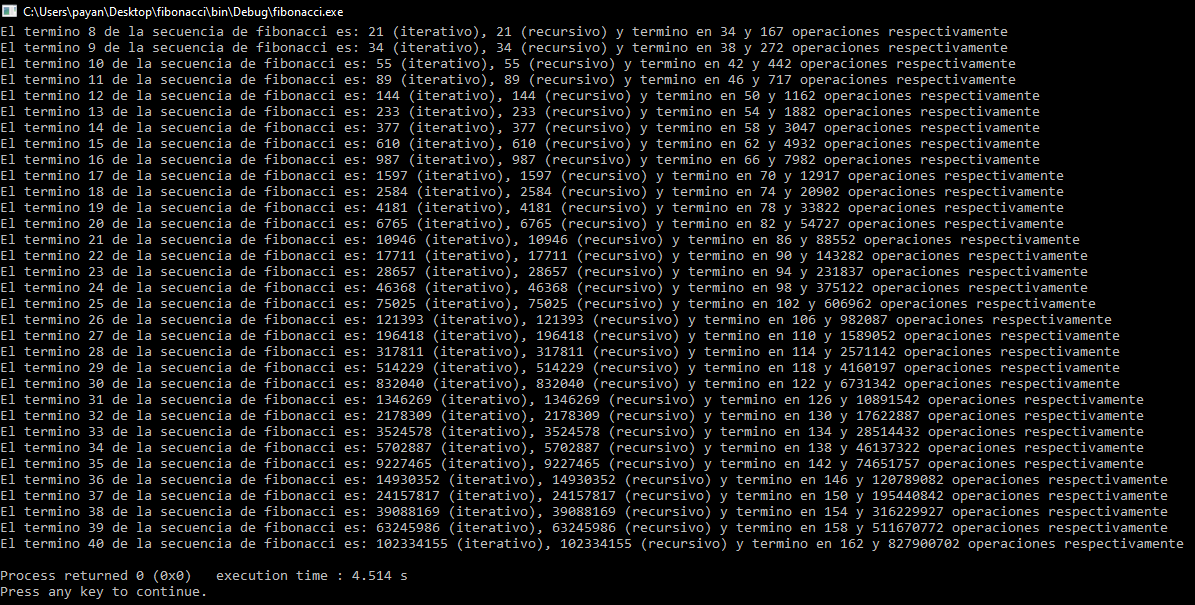
\includegraphics[width=400px,height=200px]{ejecucionPrimeraParte}
				\caption{Ejecucion del programa con ambos algoritmos, imprime $N$ y el resultado de ambas implementaciones}
			\end{figure}
			\begin{figure}[H]
				\centering
				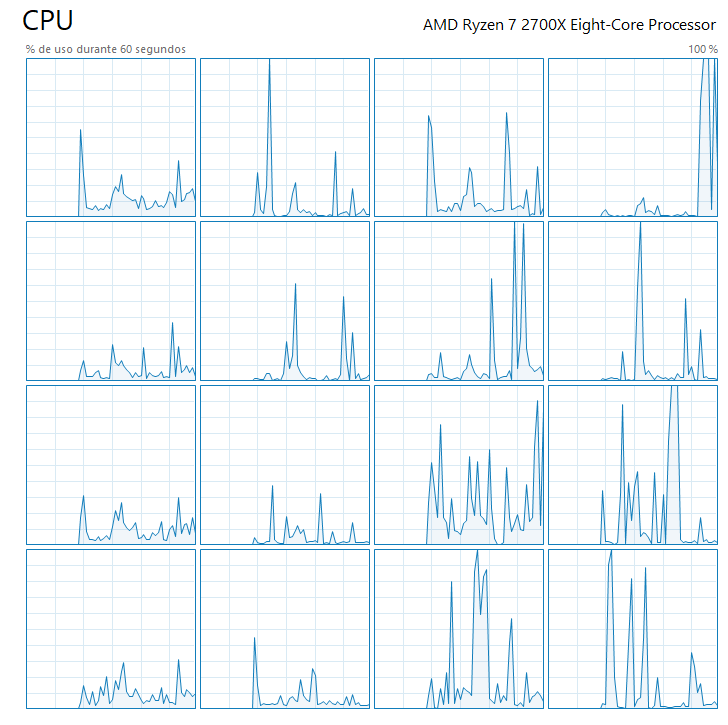
\includegraphics[width=400px,height=200px]{cpu}
				\caption{Como adicional, conforme aumentaba el valor del "limite", se incrementaba el tiempo que tardaba en terminar y el uso de CPU}
			\end{figure}
			\begin{figure}[H]
				\centering
				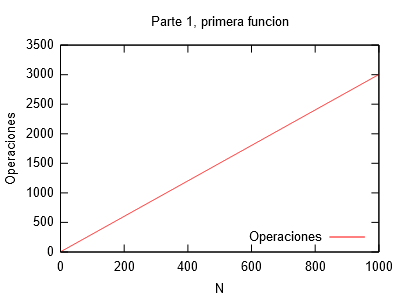
\includegraphics[width=400px,height=300px]{grafica1}
				\caption{N contra Operaciones de la solucion iterativa}
			\end{figure}
			\begin{figure}[H]
				\centering
				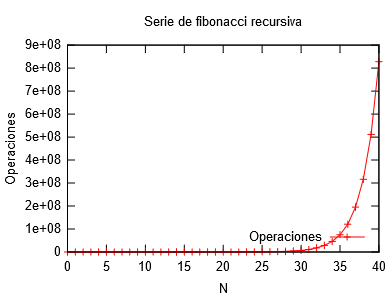
\includegraphics[width=400px,height=300px]{grafica2}
				\caption{N contra Operaciones de la solucion recursiva}
			\end{figure}
			\begin{figure}[H]
				\centering
				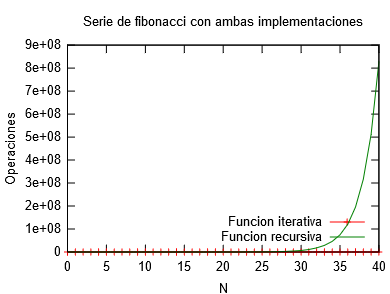
\includegraphics[width=400px,height=300px]{grafica3}
				\caption{N contra Operaciones de las dos implementaciones}
			\end{figure}
			Ahora procedemos a calcular formalmente la complejidad de la implementacion iterativa
			Empezamos calculando la complejidad temporal de cada linea:
			\begin{center}
				\begin{table}[H]
					\begin{tabular}{|l|l|l|}
						\hline
						\rowcolor[HTML]{FFCC67} 
						Codigo                           & Costo & Veces ejecutado \\ \hline
						\textit{a = 0}                    & $\O(1)$    & 1               \\ \hline
						\textit{b = 0}                    & $\O(1)$    & 1               \\ \hline
						\textit{c = 0}                    & $\O(1)$    & 1               \\ \hline						
						\textit{for(i=0;i$\leq$n;i++)} & $\O(n)$    & n+2             \\ \hline
						\textit{\  \  c = a}                 & $\O(1)$    & n               \\ \hline
						\textit{\  \  a = b}                     & $\O(1)$    & n+1               \\ \hline
						\textit{\  \  b += c}                     & $\O(1)$    & n+1               \\ \hline
						\textit{return a}                & $\O(1)$    & 1               \\ \hline
					\end{tabular}
				\end{table}										
			\end{center}			
			Lo cual nos indica que la complejidad de la solucion iterativa es lineal, es decir $T(n)\in\O(n)$. Esto lo podemos corroborar en la Figure 3 donde se puede apreciar que el numero de operaciones de la implementacion contra N crece de forma lineal.\\			
			Por otro lado, de forma experimental podemos proponer que la complejidad de la solución recursiva es: $2^N$			
		\subsection{Implementar las funciones Perfecto(N) y MostrarPerfectos(N)}
			Para el segundo conjunto de funciones, se decidio buscar los primeros 4 números perfectos, y probar todos los números hasta 10 000.
			\begin{figure}[H]
				\centering
				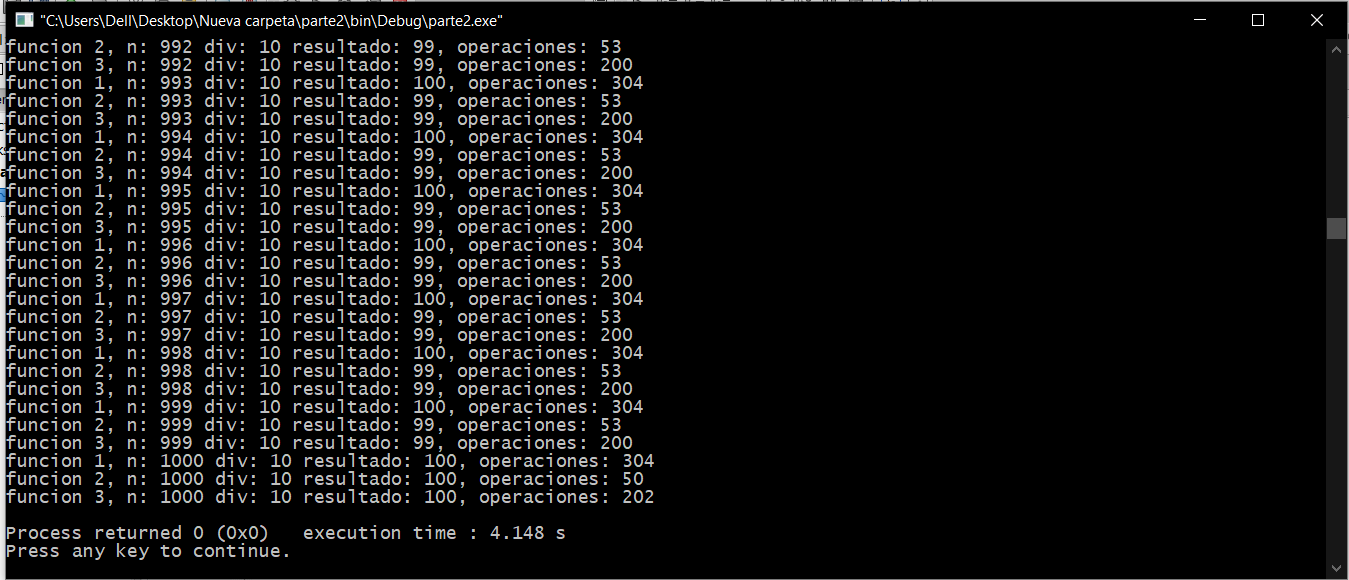
\includegraphics[width=400px,height=200px]{ejecucionSegundaParte}
				\caption{Ejecucion del programa en la seccion de prueba de números}
			\end{figure}
			\begin{figure}[H]
				\centering
				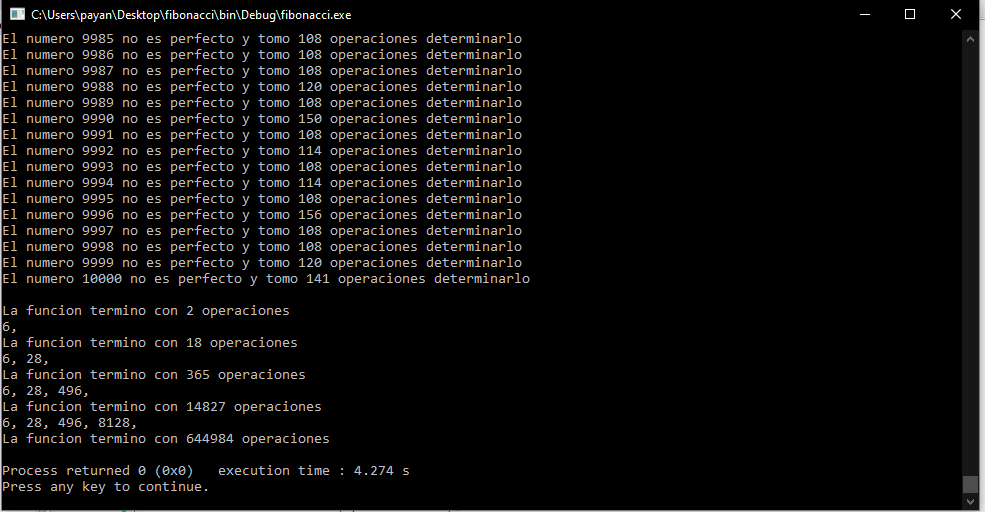
\includegraphics[width=400px,height=200px]{ejecucionTerceraParte}
				\caption{Ejecucion del programa en la seccion de obtener N perfectos}
			\end{figure}
			\begin{figure}[h!]
				\centering
				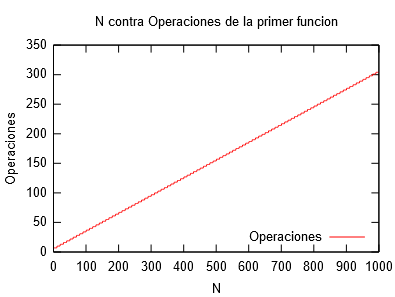
\includegraphics[width=400px,height=300px]{grafica5}
				\caption{N contra Operaciones de Perfecto(N)}
			\end{figure}
			\begin{figure}[H]
				\centering
				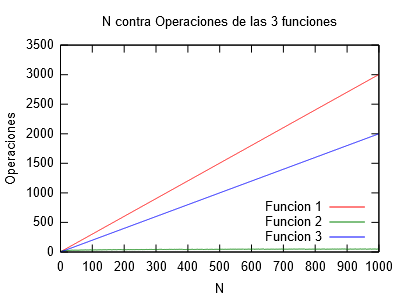
\includegraphics[width=400px,height=300px]{grafica4}
				\caption{N contra Operaciones de MostrarPerfectos(N)}
			\end{figure}
			Ahora procedemos a calcular formalmente la complejidad de la funcion Perfecto(N)
			Empezamos calculando la complejidad temporal de cada linea:
			\begin{center}
				\begin{table}[H]
					\begin{tabular}{|l|l|l|}
						\hline
						\rowcolor[HTML]{FFCC67} 
						Codigo                           & Costo & Veces ejecutado \\ \hline
						\textit{raiz = sqrt(n)}                    & $\O(1)$    & 1               \\ \hline
						\textit{suma = 1}                    & $\O(1)$    & 1               \\ \hline
						\textit{for(i=2;i$\leq$raiz;i++)} & $\O(\sqrt{n})$    & $\sqrt{n}$+2             \\ \hline
						\textit{\  \  if(n mod i == 0)}                 & $\O(1)$    & $\sqrt{n}$               \\ \hline
						\textit{\  \  \  \  if(n/i > raiz)}                     & $\O(log_2(n))$    & $log_2(n)+1$              \\ \hline
						\textit{\  \  \  \  \  \  suma += n/i}                     & $\O(1)$    & $\frac{log_2(n)}{2}$               \\ \hline
						\textit{\  \  \  \  suma+=i}                     & $\O(1)$    & $log_2(n)$               \\ \hline
						\textit{return (suma==n?1:0)}                & $\O(1)$    & 1               \\ \hline
					\end{tabular}
				\end{table}										
			\end{center}			
			Lo cual nos indica que la complejidad de la funcion Perfecto(n) es $\sqrt{n}$, es decir $T(n)\in\O(\sqrt{n})$. Esto lo podemos corroborar en la Figure 3 donde se puede apreciar que el numero de operaciones de la implementacion contra N crece acotado por abajo por $\sqrt(2)$ y acotado por arriba por $c\sqrt{n}$.\\			
			Por otro lado, de forma experimental y basado en la tabla de perfectos conocidos,podemos observar que la complejidad de la funcion MostrarPerfectos(n) crece de forma exponencial debido a que el espacio entre cada perfecto es muy grande, asimismo las formas mas optimas que ocupan el calculo de un primo p, igual tienen complejidades gigantes, debido a que es dificil hallar un primo y no todos aplican para la funcion, sin mencionar que computacionalmente cuesta muchisimo trabajo hacerlo.
			
		\section{Conclusiones}			
			\subsection{Payán Téllez René}
			Esta practica se me hizo particulamente interesante porque los algoritmos que se trataron, no fueron tan directos de implementar en un lenguaje de programación, sin mencionar que algunas graficas tuvieron muy pocos valores, debido a lo complicado que era generar mas, porque computacionalmente su complejidad es inmensa. De hecho tuve que cambiar algunas variables de int a long long int en el espacio de los contadores para que siguiera funcionando el contador sin desbordarse. Tambien vi lo interesante de un algoritmo como MostrarPerfectos que tiene una complejidad no polinomial, ya que aunque lo puedo programar tardaria horas en encontrar mas alla del perfecto 5 (de por si toma mas de 5 minutos hallar el perfecto 4) sin mencionar que le tomaria dias encontrar otros números. Tambien cuando estaba demostrando la complejidad del algoritmo recursivo de la secuencia de fibonacci, algunos nucleos del CPU de mi computadora se dispararon, lo cual fue una señal de lo complicado y tardado que se podia volver en N muy grandes.\\
			\includegraphics[height=120px,width=120px]{Rene}
		\section{Anexo}			
		\section{Bibliografia}
		{[}1{]}\url{https://openwebinars.net/blog/que-es-un-algoritmo-informatico/}\\
		{[}2{]}\url{https://medium.com/@joseguillermo_/qu%C3%A9-es-la-complejidad-algor%C3%ADtmica-y-con-qu%C3%A9-se-come-2638e7fd9e8c}\\
		{[}3{]}\url{https://es.wikipedia.org/wiki/P_(clase_de_complejidad)}\\
		{[}4{]}\url{https://es.wikipedia.org/wiki/NP_(clase_de_complejidad)}\\
		{[}5{]}\url{https://quantdare.com/numeros-de-fibonacci/}\\
		{[}6{]}\url{https://matematicascercanas.com/2015/03/04/numeros-perfectos/}\\
		{[}7{]}\url{https://www.smartick.es/blog/matematicas/numeros/numeros-primos-criba-eratostenes/}\\		
\end{document}